\documentclass[10pt,times,twocolumn]{article}

\usepackage{sbcm2019}
\usepackage{graphicx,url}
\usepackage{titling}

% -------------------------------------------------------
% Packages that facilitate double-blind peer review
% Comment the first line and uncomment the second to remove double-blindness
%\usepackage[blind]{anonymize} % Blind
\usepackage{anonymize} % not blind
% --------------------------------------------------------

%\usepackage[brazil]{babel}
%\usepackage[latin1]{inputenc}
% If needed, change this to:
 \usepackage[utf8]{inputenc}


\sloppy

\title{Baidu Search Engine}

\author{\anonymize{Chao Gao} \and
        \anonymize{Yinchu Wu} \and
        \anonymize{Peilin Wu}}


\begin{document}

\maketitle

\begin{abstract}
In this project, first we crawl Baidu Baike and Baidu Zhidao with more than 10,000 entries. We try breadth-first search strategy and best priority search strategy for web information retrieve.
Then We build inverted index from scratch based on the data. Finally, we implement a user-friendly 
frontend interface to perform queries easily.  
\end{abstract}


\section{Introduction}\label{sec:gen}
In this project, we are asked to crawl Baidu Baike (no less than 10,000 entries) and Baidu Zhidao (no less than 10,000 questions). The number of entries or questions under each category in Baidu Baike or Baidu Zhidao should be similar. For Baidu Baike, each entry includes title, subtitles and corresponding descriptions. For Baidu Zhidao, each question has different replies. There are always some images in Baidu Baike or Baidu Zhidao.

\subsection{Crawler}
Web crawlers (also known as web spiders, web bots, more often referred to as web chasers in the FOAF community) are programs or scripts that automatically crawl web information in accordance with certain rules. Other infrequently used names are ants, automatic indexes, simulators, or worms.
\begin{figure}[ht]
\centering
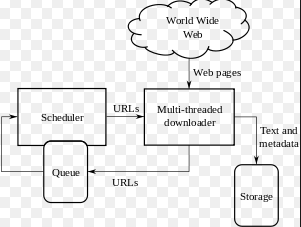
\includegraphics[scale=0.6]{fig/1.png}
\caption{a web crawler representation}
\label{fig:label}
\end{figure}
\newline
According to the system structure and implementation technology, web crawlers can be roughly divided into the following types: General Purpose Web Crawler, Focused Web Crawler, Incremental Web Crawler, Deep Network. Deep Web Crawler. The actual web crawler system is usually implemented by a combination of several crawler technologies.
\newline
The description and definition of the crawl target is the basis for determining how the web page analysis algorithm and the URL search strategy are formulated. The web page analysis algorithm and the candidate URL sorting algorithm are the key to determine the service form provided by the search engine and the crawling behavior of the crawler webpage. The algorithms of these two parts are closely related. The description of the crawl target by the existing focus crawler can be divided into three types based on the target web page feature, the target data model based on the target data model and the domain based concept.

\subsection{Search Engine}
A (web) search engine is a software system that is designed to carry out web search, which means to search the World Wide Web in a systematic 
way for particular information specified in a textual web search query. The search results are generally presented in a line of 
results, often referred to as search engine results pages(SERPs). The information may be mix of links to 
web pages, images, videos, articles and other types of files.
\begin{figure}[ht]
\centering
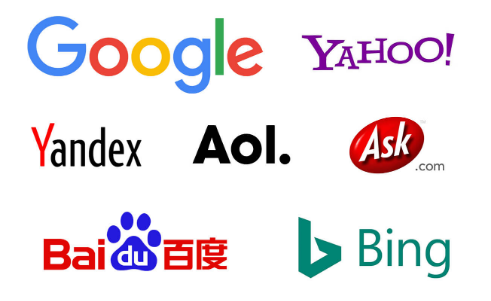
\includegraphics[scale=0.45]{fig/2.png}
\caption{popular search engines}
\label{fig:label}
\end{figure}
\newline
The first well documented search engine that searched content files, namely FTP files was \textbf{Archie}, which debuted on 10 September 1990. 
\textbf{Google} adopted the idea of selling search terms in 1998, from a small search engine company named goto.com. Around 2000, Google's search engine 
rose to prominece. In China, \textbf{Baidu} is the most popular search engine.
\newline
Based on the data crawled, indexing means associating words and other definable tokens found on web pages to their domain names and HTML-based 
fields. The associations are made in a public database, made available for web search queries. Typically when a user enters a query into search engine, 
the index already has the names of the sites containing the keywords, and these are 
instantly obtained from the index. Finally, some importance ranking algorithms are used to 
rank the results.


\subsection{Website}
A website is a collection of related network web resources, such as web pages, multimedia content which are typically with a common domain name, and published on at least one web server. \cite{wiki:website} It can be roughly divided to two different classes: static website and dynamic website.
\newline
Static websites are consists of pre-stored html pages and CCS. The content of these websites are fixed, pre-constructed by owners. Visitors can only read the content from these website. They cannot interact with these websites.
\newline
Dynamic websites , on the other side, can be interacted by users. Users might can send requests to server, create account, searching for information from these websites, depends on websites respectively. 
\newline
To implement a baidu searcher, a dynamic website is necessary. In our project,  we build a dynamic website to explicitly display the performance of our search engine.


\section{Task}
We are required to build indexes and/or other data structures to support four kinds of queries:
\begin{itemize}
    \item User asks a question like those in the Baidu Zhidao, and the system should return a ranked list of all similar questions along with their answers. If there are any Baidu Baike entries or images related to the question, the system also should return ranked lists of these entries and images. 
    \item User asks a keyword which may be any key words that might appear in the page of Baidu Baike or Baidu Zhidao, and the system returns a ranked list of related entries and a ranked list of all related questions along with their answers. If there are any related images, the system also should return a ranked list of these images. 
    \item Advanced search: let user enter search keyword for a particular region in the page, e.g., search in the Baidu Baike, the question of Baidu Zhidao, the answer of Baidu Zhidao or the images. The advance search should give the interface to allow the user to choose what region to search from. Appropriate regional/zonal indexes need to be build. 
    \item As each question in Baidu Zhidao could have different answers, you are required to delete unrelated answers and recommend a ranked list of answers. You may consider whether the answer is accepted by the question owner or the number of times the answer is considered useful.
\end{itemize}

\section{Ideas and Methods}

\subsection{Crawler Strategies}
For Baidu Baike content, we use a breadth-first search strategy. The breadth-first search strategy refers to the next level of search after completing the current level of search in the crawling process. The design and implementation of this algorithm is relatively simple. In order to cover as many web pages as possible, a breadth-first search method is generally used. There are also many studies that apply breadth-first search strategies to focused crawlers. The basic idea is that there is a high probability that a web page with a certain URL within a certain link distance has a topic relevance. Another method is to combine breadth-first search with web filtering technology, first use the breadth-first strategy to crawl web pages, and then filter out irrelevant web pages. The disadvantage of these methods is that as the number of crawled web pages increases, a large number of irrelevant web pages will be downloaded and filtered, and the efficiency of the algorithm will become lower.
\newline
For Baidu Zhidao content, we use best priority search strategy. The best priority search strategy predicts the similarity between the candidate URL and the target webpage, or the relevance to the topic according to a certain webpage analysis algorithm, and selects one or several URLs with the best evaluation to perform the crawling. It only accesses pages that have been predicted to be "useful" by web analytics algorithms. One problem that exists is that many related web pages on the crawler crawl path may be ignored because the best priority strategy is a local optimal search algorithm. Therefore, it is necessary to improve the best priority combined with the specific application to jump out of the local best. A detailed discussion will be made in conjunction with the web page analysis algorithm in Section 4. Studies have shown that such closed-loop adjustments can reduce the number of irrelevant pages by 30\% to 90\%.
\newline Finally our data is stored in \textbf{baike.csv} and \textbf{zhidao.csv}, for images, we store the mapping relationship between 
docid and the location path of images, the relation is in \textbf{images.csv}. The data format is as follows.
\begin{figure}[ht]
\centering
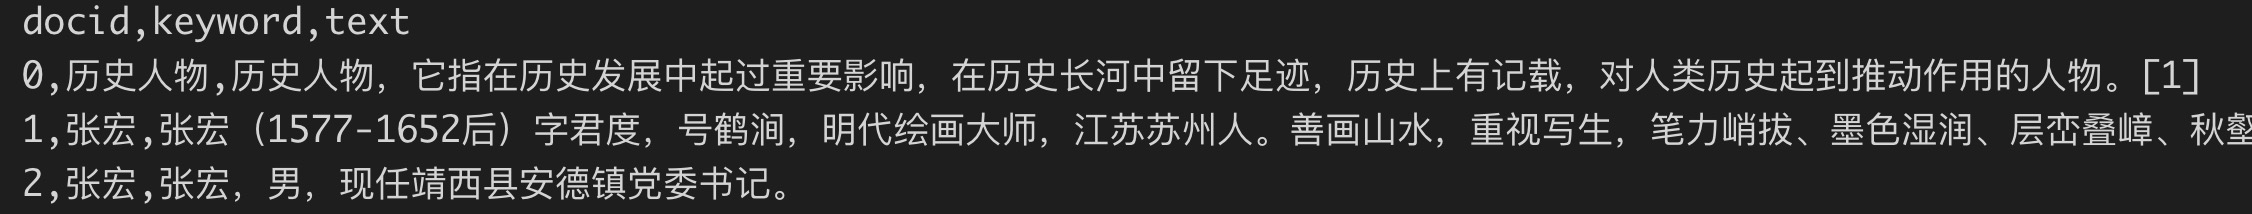
\includegraphics[scale=0.1]{fig/3}
\caption{baike data format}
\label{fig:label}
\end{figure}
\begin{figure}[ht]
\centering
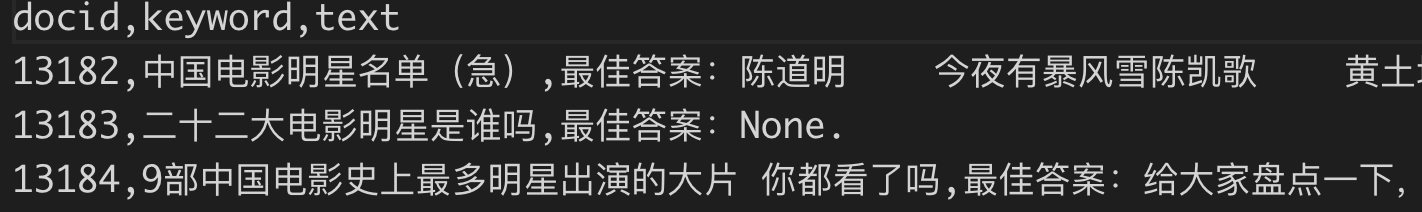
\includegraphics[scale=0.3]{fig/4}
\caption{zhidao data format}
\label{fig:label}
\end{figure}


\subsection{Search Engine}
As is known, the baike data and zhidao data actually follow the similar formats. Therefore, 
here we use the baike data as the example, and for image retrieval, we just get docids to map to the corresponding images.

\subsubsection{Indexing}
An inverted index (also referred to as a postings file or inverted file) is a database index storing a mapping from content, such as words or numbers, to its locations in a table, or in a document or a set of documents (named in contrast to a forward index, which maps from documents to content). The purpose of an inverted index is to allow fast full-text searches, at a cost of increased processing when a document is added to the database. 
\begin{figure}[ht]
\centering
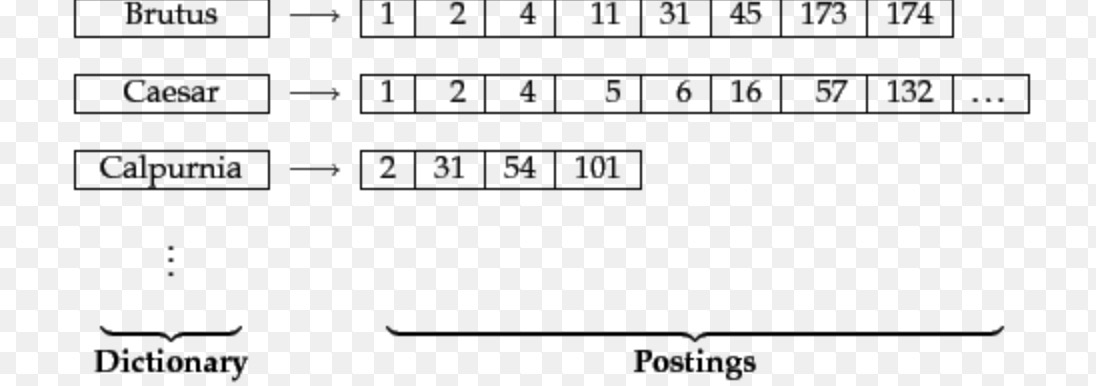
\includegraphics[scale=0.2]{fig/5}
\caption{Indexing Illustration}
\label{fig:label}
\end{figure}
\newline
Here we use \textbf{jieba} library to extract keywords from docs. When user types a query, 
we also extract keywords from the query and to find the related docs by postings.

\subsubsection{Ranking}
After we get the doc candidates, we would rank the candidates and return the most relevant docs. 
Instead of using the traditional tf-idf method, we use a better algorithm called \textbf{BM25}. BM25 (BM stands for Best Matching) is a ranking function used by search engines to estimate the relevance of documents to a given search query. It is based on the probabilistic retrieval framework developed in the 1970s and 1980s by Stephen E. Robertson, Karen Spärck Jones, and others.
\newline
BM25 is a bag-of-words retrieval function that ranks a set of documents based on the query terms appearing in each document, regardless of their proximity within the document. It is a family of scoring functions with slightly different components and parameters. One of the most prominent instantiations of the function is as follows.
\newline
Given a query Q, containing keywords {$q_{1}$,...,$q_{n}$}, the BM25 score of a document D is:
\begin{equation}
    s=\\ \sum_{i=1}^{n}{IDF(q_i)\frac{f(q_i, D)\cdot (k_1+1)}{f(q_i+D)+k_1\cdot (1-b+b\cdot\frac{|D|}{avgdl})}}
\end{equation}
Where $f(q_i, D)$ is $q_i's$ term frequency in the document D, |D| is the length of the document D in words, 
and avgdl is the average length in the text collection from which documents are drawn. $k_{1}$ and b are free parameters. IDF($q_i$) is the IDF (inverse document frequency) weight of the query term $q_{i}$, 
it is usually computed as:
\begin{equation}
    IDF(q_i)=log\frac{N-n(q_i)+0.5}{n(q_i)+0.5}
\end{equation}
Where $N$ is the total number of documents in the collection, and 
$n(q_i)$ is the number of documents containing $q_i$.
\subsection{Website}
Our searcher consists of four different template pages: index page, search page, baike page and zhidao page. 
\newline
For index page, it shows our searcher’s logo as well as give a input box to users to enter the keywords which they want to search. Besides, it provides three checked boxes for users to let them choose the coverage of the searching.  When users send searching request, it send the keywords and the status of each checked boxes to the server. Then the server will parse the keyword, use the methods described in section 3.2 and uses the searching result to construct search page. Eventually, searching results are shown to user in search page.
\newline
For search page, it contains all components in index page, but in another form. It also displays the searching results from users’ input keywords, including images and links. To implement webpages in a  dynamic way,  a framework in Python3, flask and Jinja2 syntax is used in our website. By using them, if-statement and for-loop can be implemented in html, which makes things much easier. Besides, Bootstrap is used in template pages to design the webpages. 
\newline
Each link in the searching result has its own globally identity. When users click a link in the searching result, search page sends the link’s identify to the server. The server then sends back all information needed to construct this baike or zhidao page. Eventually, all the results will be put on corresponding pages.


\section{Result}

To show the preformance of our baidu searcher, we choose some examples queries and search the result in different condition. 
\newline
Figures below shows the results from searching a keyword.
\begin{figure}[ht]
\centering
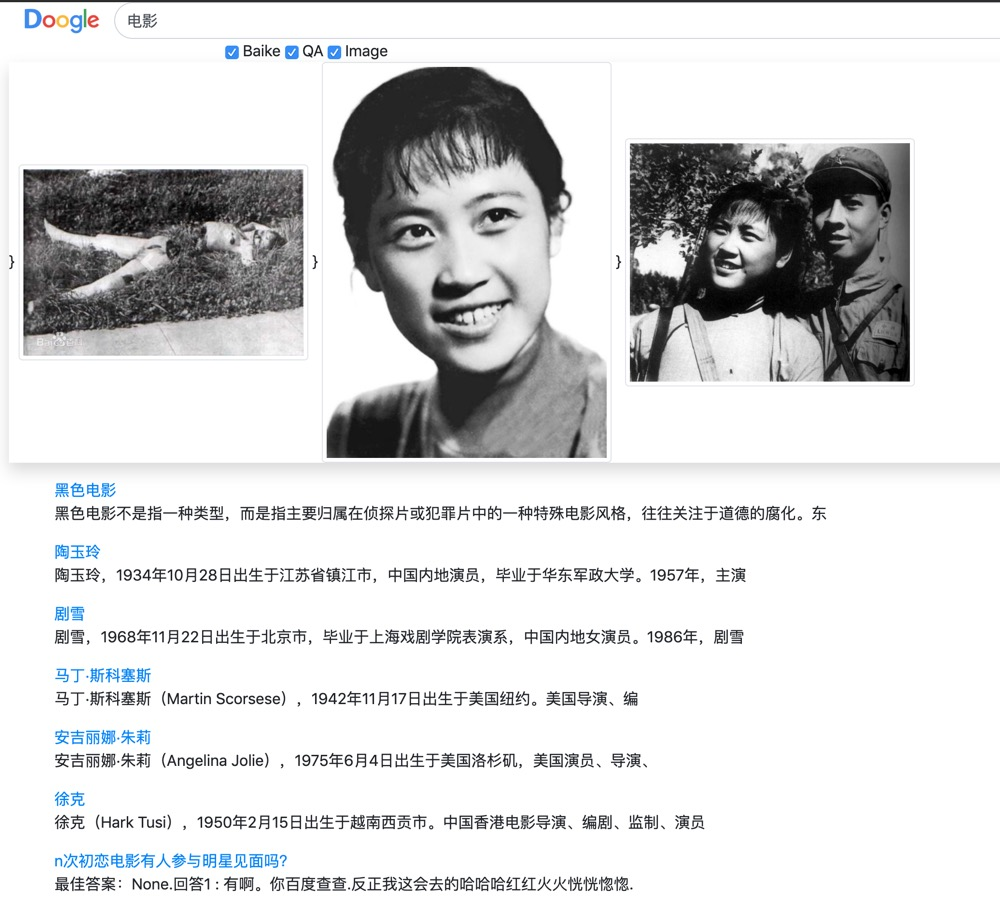
\includegraphics[scale=0.2]{fig/6}
\caption{result for a keyword}
\label{fig:label}
\end{figure}
\newline
Also we can type a question.
\begin{figure}[ht]
\centering
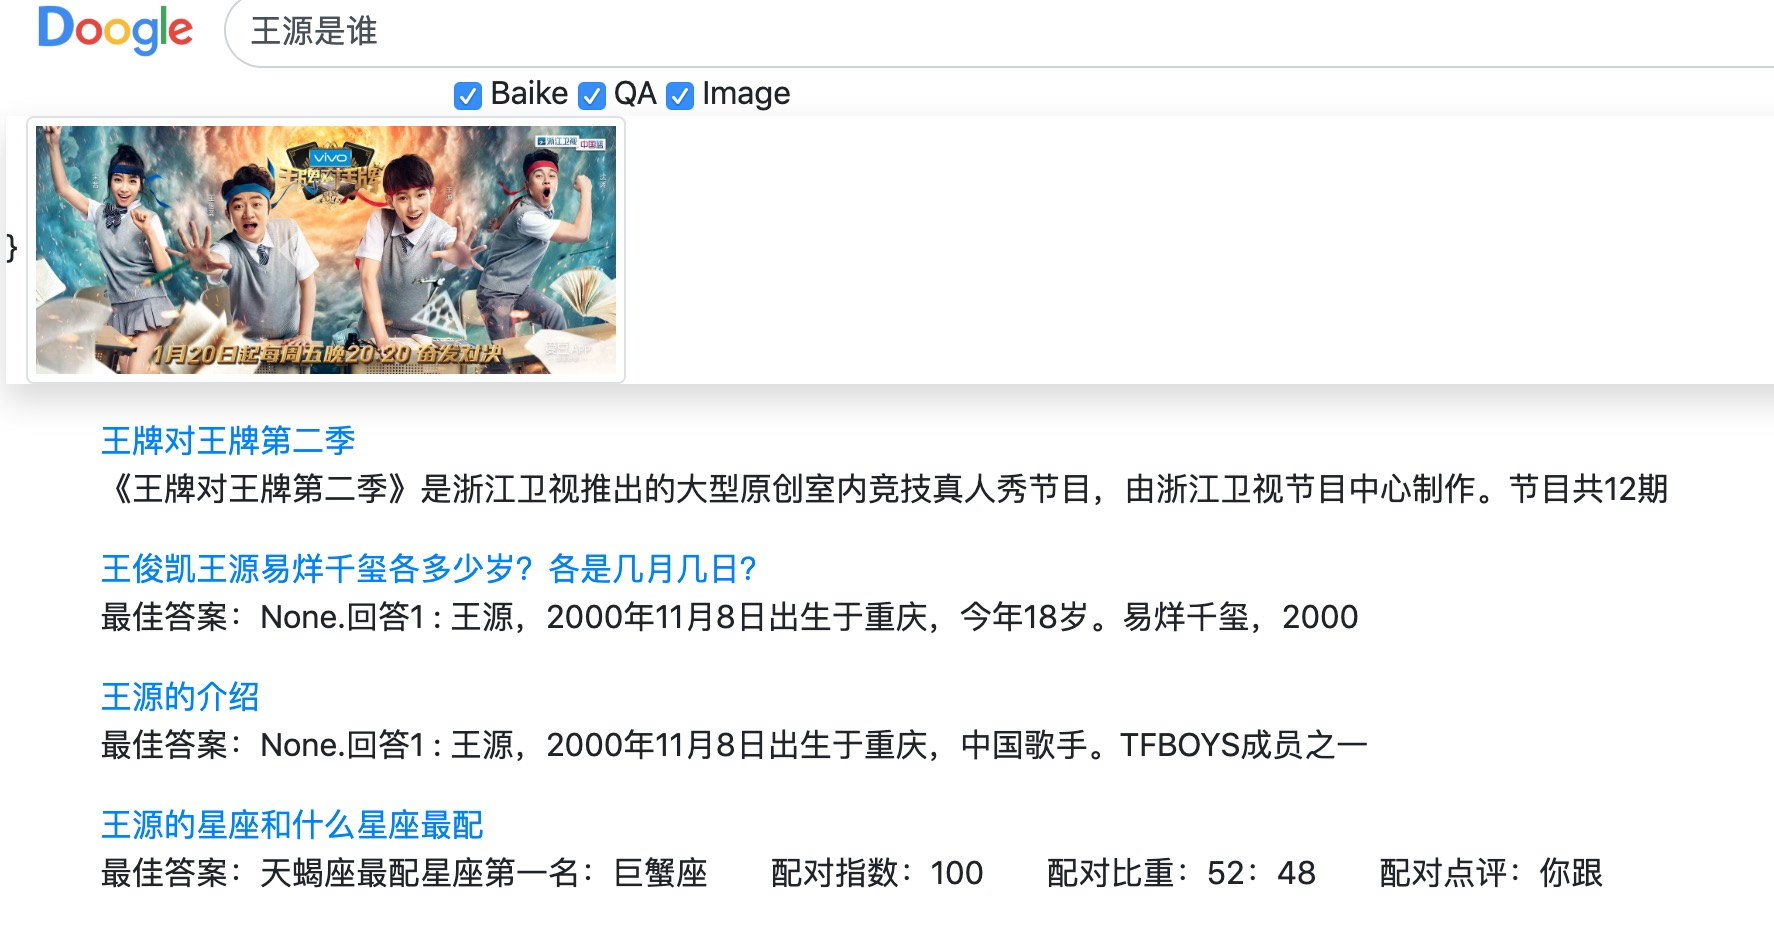
\includegraphics[scale=0.13]{fig/7}
\caption{result for a question}
\label{fig:label}
\end{figure}
\newline
We can limit the coverage of this query to baike, the results are shown below:
\begin{figure}[ht]
\centering

\includegraphics[scale=0.1]{fig/8}
\caption{baike result}
\label{fig:label}
\end{figure}
\newline
Also we can click the link to see the whole content.
\begin{figure}[ht]
\centering
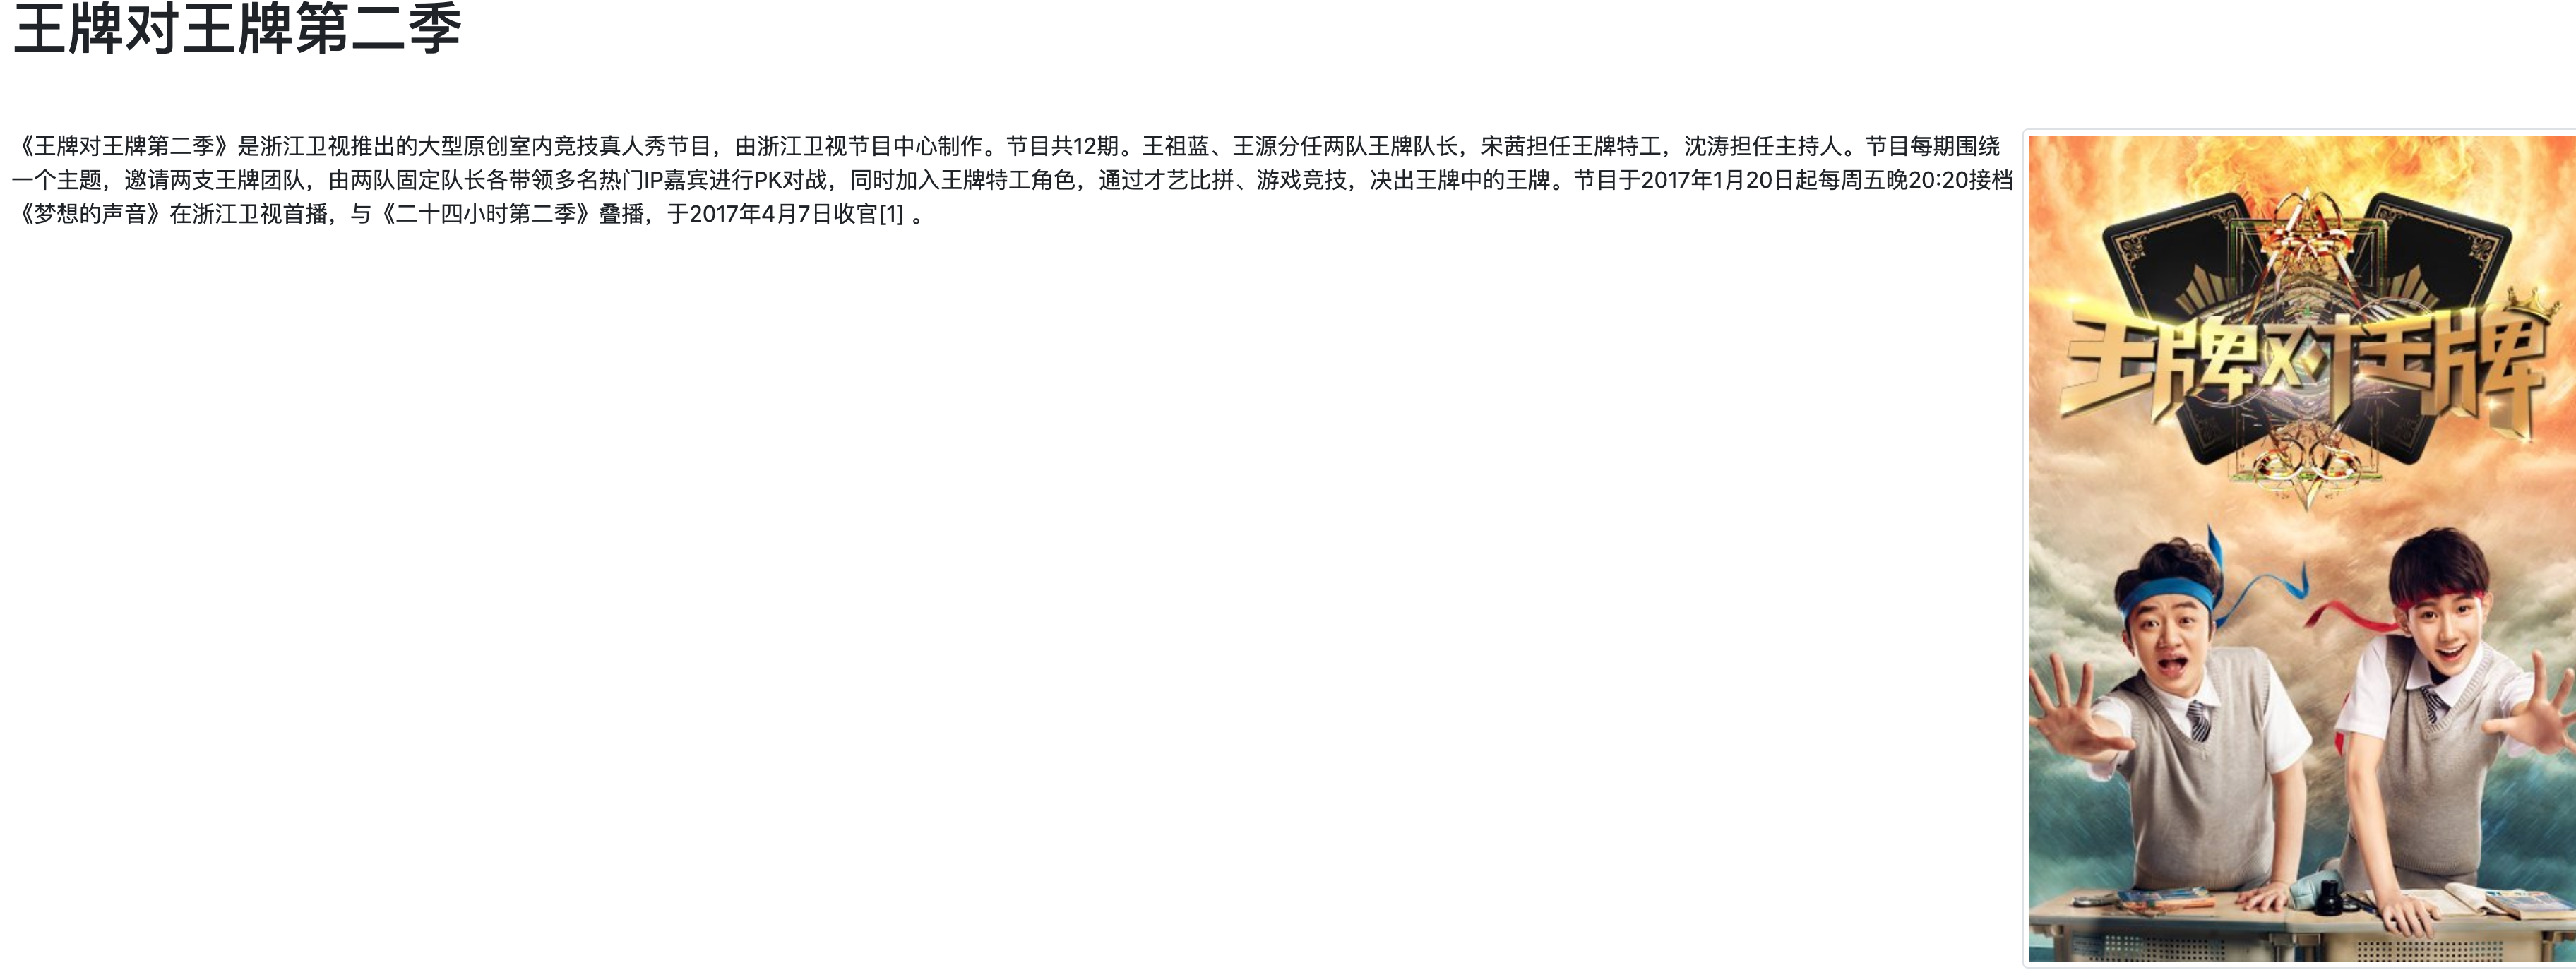
\includegraphics[scale=0.1]{fig/9}
\caption{baike whole content}
\label{fig:label}
\end{figure}
We can also limit the coverage of this query to baike, the results are shown below:
\begin{figure}[ht]
\centering
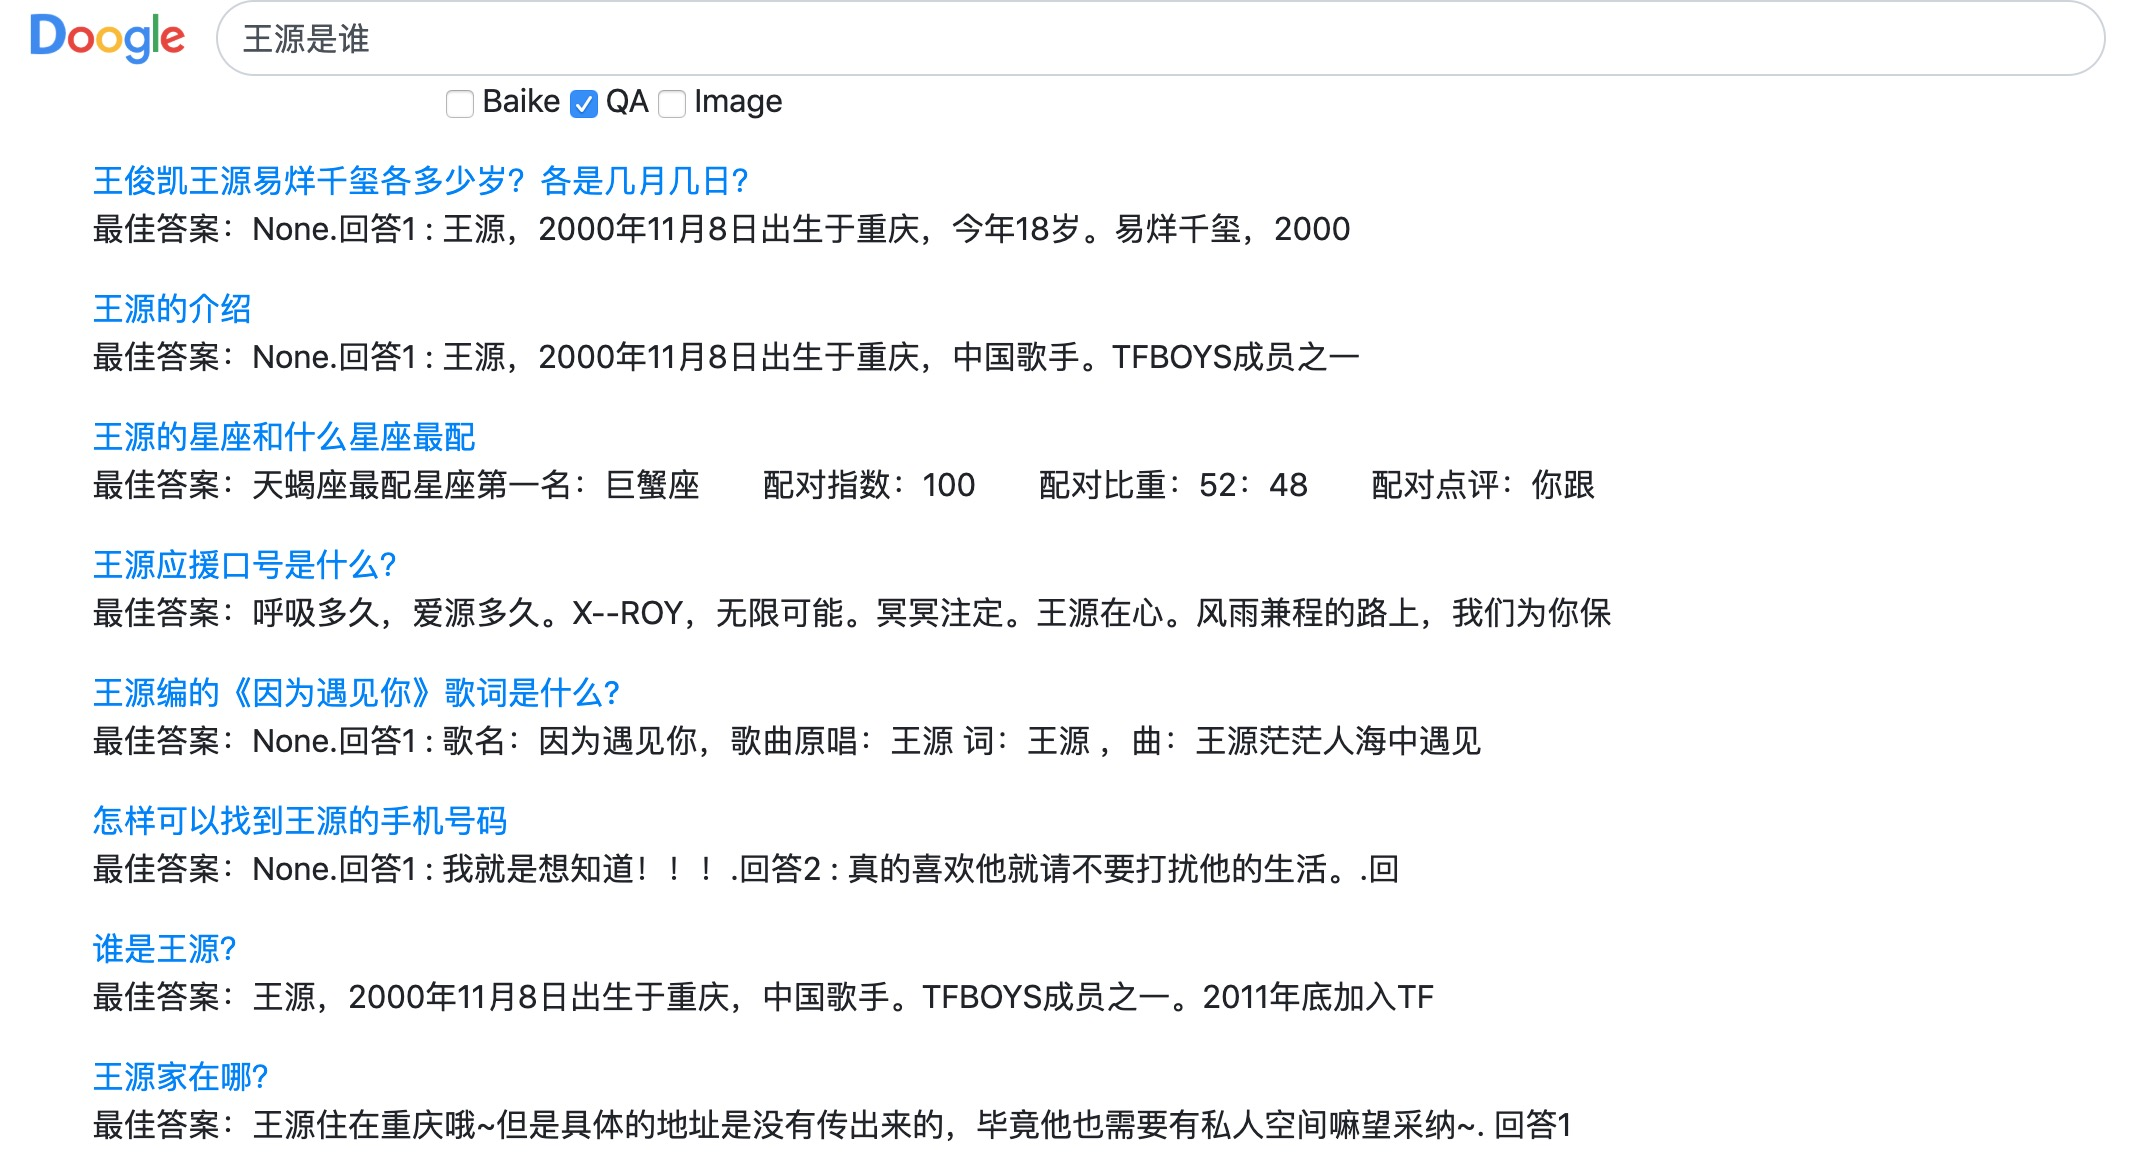
\includegraphics[scale=0.13]{fig/10}
\caption{zhidao result}
\label{fig:label}
\end{figure}
\newline
Similar to baike, we can also see the whole content of zhidao.
\begin{figure}[!h]
\centering
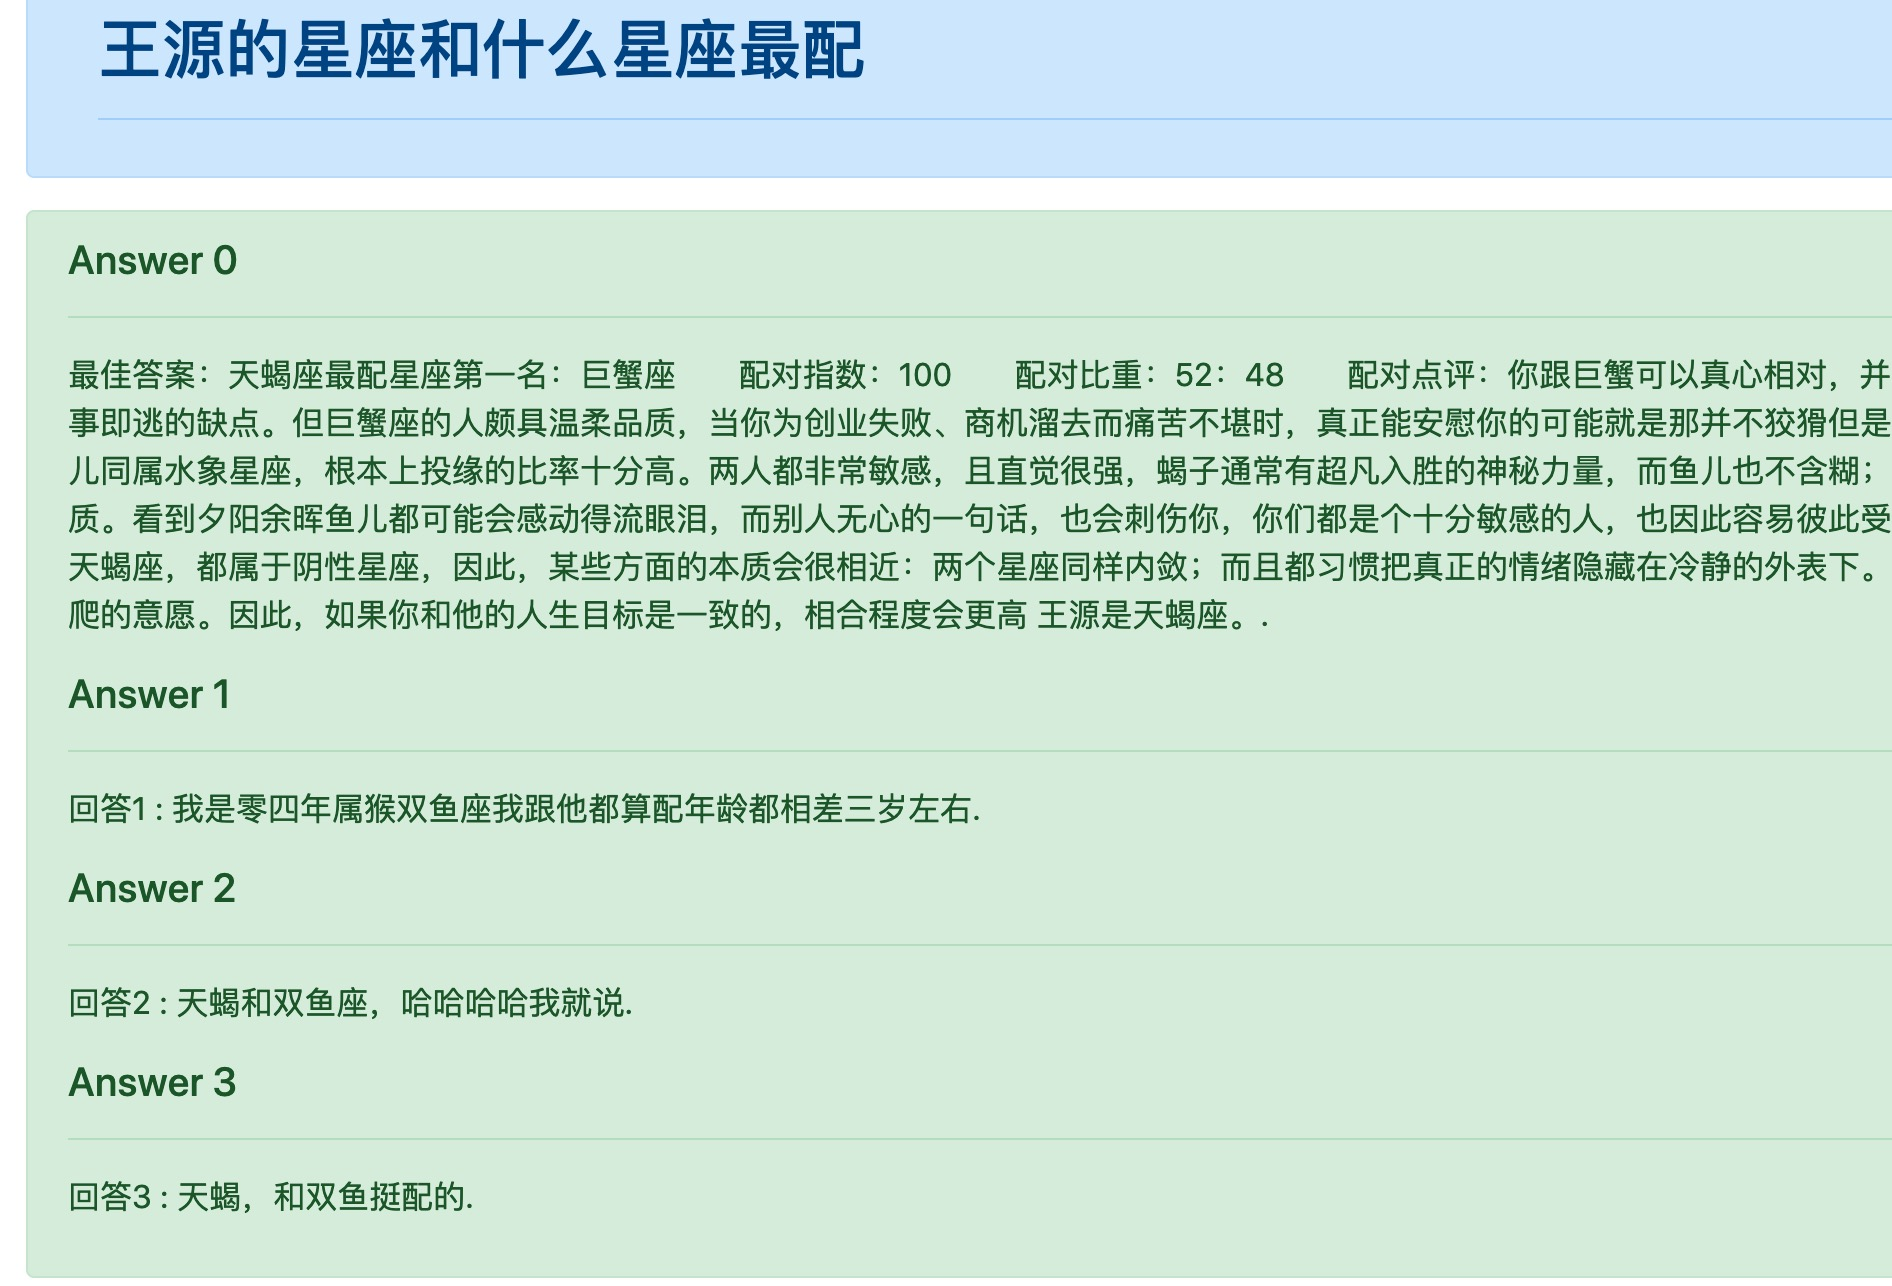
\includegraphics[scale=0.13]{fig/11}
\caption{zhidao whole content}
\label{fig:label}
\end{figure}
\newline
We can also limit the coverage of this query to images, the result are as follows.
\begin{figure}[h]
\centering
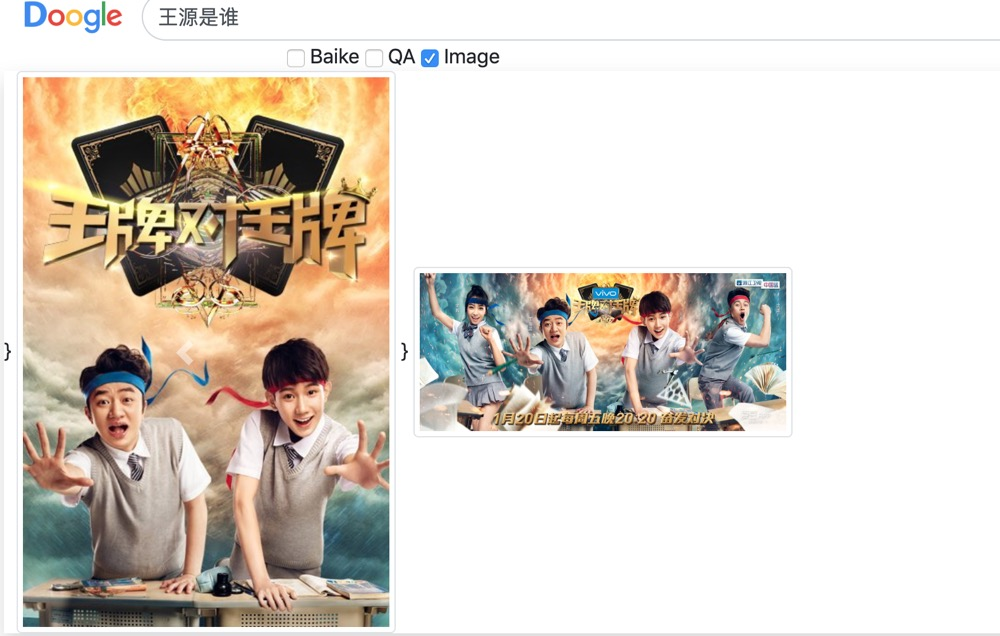
\includegraphics[scale=0.1]{fig/12}
\caption{image result}
\label{fig:label}
\end{figure}

\section{Conclusion}
In this project, we have learned a lot in writing a web crawler. And what's more, we also implement the indexing 
and ranking algorithm learned from class and Internet by ourselves, without using any open-source retrieval libraries. 
Also, we pay lots of attention on UI design to make it easier and intuitive for users to use.
\section{Acknowledgments}
We are very grateful to the teachers and TAs for their help during this semester. 

% \bibliographystyle{unsrt}
% \bibliography{example}

\end{document}

